\documentclass[a0paper,portrait,margin=0pt, colspace=24pt,subcolspace=0pt,blockverticalspace=36pt,innermargin=30pt]{tikzposter}

\usepackage[latin9]{inputenc}
\usepackage{cite}
%\usepackage[square,numbers]{natbib} 	% Bibliography manager
\usepackage{amsmath,amssymb}
\usepackage{lipsum}  				    % Random Text
\usepackage[colalign]{aligncolsatbottom}  %To align columns at bottom (!! please run 2 times)
\usepackage[inline,shortlabels]{enumitem}

%..............................................................................................................................................................................................
% Display
\tikzposterlatexaffectionproofoff 			
\usetikzlibrary{shapes.geometric,arrows.meta,positioning}  %Tikz Libraries

% Fonts
\usepackage{helvet}					% Sans-Serif
\renewcommand{\familydefault}{\sfdefault}	%

% Colors
\definecolor{MyGreenD}{RGB}{48, 209, 88}
\definecolor{MyRedD}{RGB}{225, 69, 58}
\definecolor{MyBlueD}{RGB}{10, 132, 255}
\definecolor{MyYellowD}{RGB}{255, 214, 10}
\definecolor{MyOrangeD}{RGB}{255, 159, 10}
\definecolor{MyWhiteD}{RGB}{142, 142, 147}
\definecolor{MyWhite2D}{RGB}{99, 99, 102}
\definecolor{MyBlackD}{RGB}{44, 44, 46}
\definecolor{MyBlack2D}{RGB}{28, 28, 30}

\definecolor{MyGreenL}{RGB}{52, 199, 89}
\definecolor{MyRedL}{RGB}{225, 59, 48}
\definecolor{MyBlueL}{RGB}{0, 122, 255}
\definecolor{MyYellowL}{RGB}{255, 204, 0}
\definecolor{MyOrangeL}{RGB}{255, 149, 0}
\definecolor{MyWhiteL}{RGB}{242, 242, 247}
\definecolor{MyWhite2L}{RGB}{229, 229, 234}
\definecolor{MyBlackL}{RGB}{147, 147, 148}
\definecolor{MyBlack2L}{RGB}{142, 142, 147}

% Theme
\usetheme{Default}
\definecolorstyle{MyStyle2016}{
	\definecolor{ColorOne}{named}{MyBlackL} 
	\definecolor{ColorTwo}{named}{MyBlueL}
	\definecolor{ColorThree}{named}{MyRedL}
}{
    % Title Colors
    \colorlet{titlebgcolor}{MyWhite2L}
    \colorlet{titlefgcolor}{MyBlueL}
    % Background Colors
    \colorlet{backgroundcolor}{MyBlackL}
    \colorlet{framecolor}{MyBlackL}
    % Block Colors
    \colorlet{blocktitlebgcolor}{MyWhite2L}
    \colorlet{blocktitlefgcolor}{MyBlueL}
    \colorlet{blockbodybgcolor}{MyWhite2L}
    \colorlet{blockbodyfgcolor}{MyWhite2D}
    % Innerblock Colors
    \colorlet{innerblocktitlebgcolor}{MyWhite2L}
    \colorlet{innerblocktitlefgcolor}{MyBlueL}
    \colorlet{innerblockbodybgcolor}{MyWhite2L}
    \colorlet{innerblockbodyfgcolor}{MyWhite2D}
    % Note colors
    \colorlet{notebgcolor}{MyBlueL}
    \colorlet{notefgcolor}{MyBlueL}
    \colorlet{notefrcolor}{MyBlueL}
 }

% Color style
\usecolorstyle{MyStyle2016}

\renewcommand{\labelitemi}{$\textcolor{MyBlueL}{\bullet}$}
\renewcommand{\labelitemii}{$\textcolor{MyBlueL}{\bullet}$}

%..............................................................................................................................................................................................
\title{\textbf{The Best Title Ever}}

\author{\textcolor{MyWhite2D}{Presenting Author and Second Author}}

\institute{\textcolor{MyWhite2D}{Institute}}

%..............................................................................................................................................................................................
\begin{document}
%
%
%	HEAD
%
%....................................................................................
%
%	Title
%
\maketitle[width=0.98\linewidth,titletoblockverticalspace=36pt,linewidth=0,roundedcorners=16]
%..............................................................................................................................................................................................
%
%	LEFT COLUMN
%
\begin{columns}
\column{0.33}
%....................................................................................
%
%	Block
%
\block[titleleft,roundedcorners=16]{Introduction}{
	\raggedright
	\lipsum[4]
}
%....................................................................................
%
%	Block
%
\block[titleleft,roundedcorners=16]{First Block}{
	\raggedright
	\lipsum[12]
}
%....................................................................................
%
%	Block
%
\block[titleleft,roundedcorners=16]{Model Block}{
	\lipsum[12]
	 
 	That was a flowchart, and this is the corresponding ODE system:
	 
	\primary{
	\[
	\left\{
	\begin{aligned}
	    \dot{S} & =  \pi - \alpha S,\\ 
	    \dot{I}  & =   \alpha S - \beta I,\\
	    \dot{R} & = \beta I - \mu R. \\
	\end{aligned}
	\right.
	\]
	 }
	 \begin{definition}{Theorem name}
	test theorem\cite{Source1}
	\end{definition}
	\begin{assumption}{Theorem name}
	test theorem
	\end{assumption}
	\begin{remark}{Theorem name}
	test theorem\cite{Source2}
	\end{remark}
	\begin{example}{Theorem name}
	test theorem
	\end{example}
}
%..............................................................................................................................................................................................
%
%	CENTER COLUMN
%
\column{0.34}
%....................................................................................
%
% 	Block
%
\block[titleleft,roundedcorners=16]{Results Block}{
	\raggedright
	This graphic was generated with Tikz:
	
	\begin{center}
	\begin{tikzpicture}[xscale=1.5,yscale=4,line width=4pt,text=ColorTwo]
		\draw [very thin, gray,step=0.5] (-pi,-1) grid (pi,1);
		\draw [color=ColorThree,domain=-pi:pi] plot (\x,{sin(\x r)});
		\draw (pi,0) node[right]{$\sin(x)$} ;
	\end{tikzpicture}
	 \end{center}

	\raggedright
	\lipsum[85]
	
	
	\vspace{3cm}
	
	\lipsum[85]
	
	\begin{itemize}
	\item Test\cite{Source3}
	\begin{itemize}
	\item Test
	\end{itemize}
	\item test
	\end{itemize}
 }
%....................................................................................
%
%	Block
%
\block[titleleft,roundedcorners=16]{Another Block}{
	\raggedright
	\lipsum[13]
	\vspace{3cm}
	\begin{theorem}{Theorem name}
	test theorem
	\end{theorem}
	\begin{corollary}{Theorem name}
	test theorem
	\end{corollary}
	\begin{proposition}{Theorem name}
	test theorem\cite{Source4}
	\end{proposition}
	\begin{lemma}{Theorem name}
	test theorem
	\end{lemma}
}
%..............................................................................................................................................................................................
%
% 	RIGHT COLUMN
%
\column{0.33}
%%....................................................................................
%
%	Block
%
\block[titleleft,roundedcorners=16]{Another block}{
	\raggedright
	
	\lipsum[85]
	\begin{center}
	\begin{figures}
    	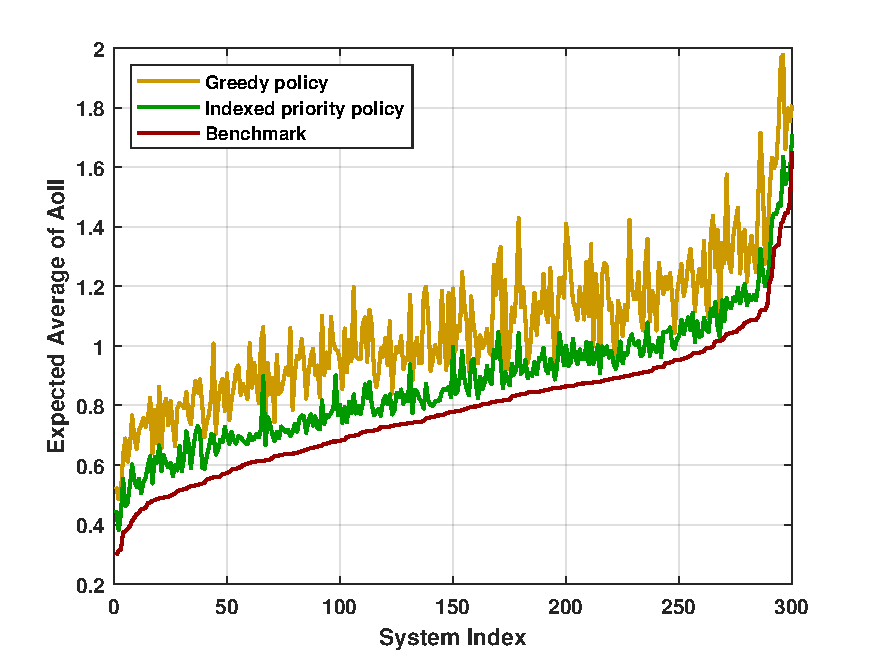
\includegraphics[width=\linewidth]{Figures/Random.pdf}
	\end{figures}
	\blue{Figure:} Random system settings
	\end{center}
	
	}
%....................................................................................
%
%	Block
%
\block[titleleft,roundedcorners=16]{Conclusions}{
	\raggedright
	\lipsum[12-13]
	\begin{itemize}
	\item Test\cite{Source3}
	\item test
	\end{itemize}
 }
\end{columns} 
%..............................................................................................................................................................................................
%
%	FOOT
%
%....................................................................................
%
%	References
%
\block[titleleft,roundedcorners=16]{}{
\small
\begin{minipage}{\linewidth}
	\nocite{*}
	\bibliographystyle{plain}
	\bibliography{Mybib}
 \end{minipage}
}

%....................................................................................
%
%	Logo & Info
%
\block[titleleft,roundedcorners=16]{}{
\begin{minipage}[b]{0.33\linewidth}
	\nocite{*}
	\textbf{Contact Information:}\\
	Email: \texttt{cheny@umd.edu}\\
	Phone: +1 (xxx) xxx xxxx
\end{minipage}
\begin{minipage}[b]{0.33\linewidth}
\centering
	%\includegraphics[height=4cm]{Figures/xxx.png}
\end{minipage}
\begin{minipage}[b]{0.33\linewidth}
\centering
	%\includegraphics[height=4cm]{Figures/xxx.png}
\end{minipage}
}

\end{document}